\documentclass[twoside,11pt]{article}
\usepackage[english]{babel}
\usepackage[utf8]{inputenc}
\usepackage[T1]{fontenc}
\usepackage{amsmath,amssymb,amsfonts,amsthm}
\usepackage{graphicx}
\usepackage{float}
\usepackage{epsfig}
\usepackage{array}
\usepackage{url}
\usepackage{hyperref}
\usepackage{orcidlink}

\textwidth=155mm
\textheight=233mm
\voffset=-15mm
\oddsidemargin=0mm
\evensidemargin=0mm
\setlength{\parindent}{6mm}
\setlength{\parskip}{0pt}
\clubpenalty=10000
\widowpenalty=10000
\displaywidowpenalty=10000
\raggedbottom
\sloppy

\newtheorem{definition}{Definition}[section]
\newtheorem{remark}{Remark}[section]
\providecommand{\R}{\mathbb{R}}

\pagestyle{myheadings}
\markboth{\hfill{\footnotesize\rm Koshikov and Tutkyshbayeva}\hfill}
{\hfill{\footnotesize\sl ML model for real-time programming feedback}\hfill}

\begin{document}
\thispagestyle{empty}
\begin{flushleft}
{\small {\bf EURASIAN JOURNAL OF MATHEMATICAL\\ AND COMPUTER APPLICATIONS}\\
ISSN 2306--6172\\
Volume 14, Issue (2026) \_ -- \_}
\end{flushleft}
\vskip 5 mm

\centerline{\bf A MACHINE LEARNING MODEL FOR REAL-TIME}
\centerline{\bf PERSONALIZED FEEDBACK IN INTRODUCTORY PROGRAMMING}

\vskip 0.2cm
\centerline{\bf Koshikov A. \orcidlink{0009-0003-3234-6487}, Tutkyshbayeva S. \orcidlink{0000-0002-1419-2571}}

\vskip 0.2cm
\noindent{\bf Abstract}
{\small
Virtual mentors for novice programmers need a reliable decision layer before they generate feedback. This paper studies that layer as a machine learning model for real-time personalized support in introductory programming. The model is implemented in SocratesAI, a web-based prototype that connects code submission, feedback-state prediction, feedback generation, and interaction logging. A public dataset of Python Codeforces submissions was filtered to beginner-level problems and converted from judge outcomes into five feedback states: accepted, semantic debugging, execution safety, efficiency review, and syntax repair. The frame contains 178414 submissions from 872 problems and is evaluated on unseen problems. A source-code model using hashed character n-grams achieved macro $F_1=0.426$, compared with $0.085$ for the majority baseline. A model that also uses run results achieved macro $F_1=0.814$. The results show when early code-only estimates are useful and when the mentor should wait for run results.}

\vskip 0.2cm
\noindent{\bf Key words:} virtual mentor, programming education, machine learning, automated feedback, Codeforces, problem-level evaluation
\vskip 0.2cm
\noindent{\bf AMS Mathematics Subject Classification:} 68T05, 68N19, 97Q60

\vskip 0.2cm
\noindent{\bf DOI:} To be assigned.
\vskip 0.3cm

\section{\large Introduction}

The practical difficulty in a programming mentor is often not the last step, where a message is written for the student. The harder part is the decision immediately before that: whether the attempt should be treated as a correct solution, a syntax problem, a runtime failure, an inefficient algorithm, or a deeper semantic error. For a first-year student these cases should lead to different kinds of support. A syntax failure usually needs a localized repair hint. A time limit failure usually needs a question about algorithmic complexity. A wrong answer may require a test-case oriented debugging prompt instead of another explanation of the whole topic.

Many recent systems for programming education use large language models to produce feedback text \cite{Denny2024,Ahamed2025,CodeAid2024,Iris2024}. This is useful, but it can hide the smaller modelling problem that decides the pedagogical state of a submission. If that decision is shallow, the generated text also becomes shallow: the mentor may sound fluent while reacting to the wrong signal. For this reason, the present work focuses on the machine learning layer that classifies the feedback need before natural-language feedback is produced.

The scope is intentionally narrower than a complete tutoring system. The study uses real programming submissions and official judge outcomes, but it does not claim to measure classroom learning gains. The aim is to build and evaluate a model that can support a virtual mentor by predicting a compact feedback state from a student's code and, when available, run results. SocratesAI is the implementation context for this model: a student writes code, the backend calls the ML service, the feedback layer prepares a bounded hint or question, and the prediction is saved for later analysis.

Accordingly, the contribution is the learned decision model: the representation, label definition, problem-level evaluation, and remaining error structure. The interface, response time, and generated text are deployment context.

The paper is guided by three research questions about generalization, evidence, and use inside SocratesAI.

\begin{itemize}
\item {\bf RQ1.} Can a learned feedback-state model generalize to submissions from beginner-level problems that were not used during training?
\item {\bf RQ2.} How much does prediction quality improve when source code is combined with run results such as passed tests, time, and memory?
\item {\bf RQ3.} Which feedback states remain unreliable, and how should SocratesAI handle low-confidence predictions through confidence scores and interaction logging?
\end{itemize}

The main contributions are as follows. First, the paper formulates an outcome-based feedback-state taxonomy suitable for introductory programming feedback. Second, it evaluates machine learning models on 178414 real submissions with a problem-level train-test split. Third, it reports an ablation over source code, problem context, static code metrics, and run results. Fourth, it connects the empirical findings to the implemented SocratesAI decision layer, where predictions and outcomes are stored in \hbox{interaction\_logs} for later classroom validation.

All reported decision models are trained estimators. The only non-learning baseline is the majority classifier, included to show how much of the result is due to the class distribution. The paper therefore studies the ML feedback-state layer directly, rather than the surrounding application workflow.

\section{\large Related work}

Automated assessment and feedback for programming has a long history, and recent surveys describe both the usefulness and the limitations of current tools \cite{Messer2024,Kumar2025}. Traditional automated graders can mark correctness reliably, but a virtual mentor needs a more careful intermediate representation: it must know what type of help should be given and how much help is appropriate.

The recent growth of LLM-based teaching assistants has made this question more visible. Denny et al. discuss desirable characteristics of AI teaching assistants in programming education, including reliability, usefulness, and alignment with learning goals \cite{Denny2024}. CodeAid studies a classroom deployment that balances student and educator needs \cite{CodeAid2024}. Iris presents an AI-driven virtual tutor for computer science education \cite{Iris2024}. Ahmed et al. study the feasibility of augmenting teaching assistants with AI for CS1 feedback \cite{Ahamed2025}. These works show that feedback quality is not only a natural-language generation problem; it also depends on when the system intervenes and what kind of intervention it chooses.

Other studies focus on student behaviour around AI help. Sheese et al. analyse patterns of help-seeking with an LLM-powered programming assistant \cite{Sheese2024}. Marwan et al. show that immediate adaptive feedback can support programming learning when feedback is designed around the learner's current state \cite{Marwan2022}. These results motivate the present paper's narrower modelling goal: before a mentor writes a hint, it should estimate the current feedback need from observable evidence.

The machine learning part of this work follows a standard supervised text-classification pipeline with sparse code features. Scikit-learn is used for reproducible modelling \cite{Pedregosa2011}, and feature hashing is used to represent character n-grams without building a large vocabulary \cite{Weinberger2009}. The empirical data come from a public Codeforces Python submissions dataset \cite{MatrixStudio2026}. Low-rated filtering keeps the dataset close to introductory attempts while preserving objective outcomes.

\section{\large Problem formulation}

Let
\[
D=\{(x_i,y_i,g_i)\}_{i=1}^{n}
\]
be a dataset of programming submissions. Here $x_i$ is the observable submission information, $y_i$ is the feedback state, and $g_i$ is the problem identifier. The feature vector is written as
\[
x_i=(c_i,m_i,e_i),
\]
where $c_i$ is the source code, $m_i$ contains problem and static-code metadata, and $e_i$ contains optional execution signals. In the source-only setting, $e_i$ is not used.

\begin{definition}
A feedback state is a discrete class that describes the type of intervention required for a submission. In this paper the label set is
\[
Y=\{\hbox{accepted},\hbox{semantic\_debug},\hbox{execution\_safety},
\hbox{efficiency\_review},\hbox{syntax\_repair}\}.
\]
\end{definition}

The states are built from official judge outcomes. The mapping is shown in Table \ref{tab:taxonomy}. The mapping should not be read as a teacher-written hint. It is an operational target for the decision layer: it tells the mentor what kind of feedback route is likely to be relevant.

\begin{table}[H]
\centering
\small
\caption{Outcome-based feedback-state taxonomy.}
\label{tab:taxonomy}
\begin{tabular}{|>{\raggedright\arraybackslash}p{35mm}|>{\raggedright\arraybackslash}p{48mm}|>{\raggedright\arraybackslash}p{58mm}|}
\hline
{\bf Feedback state} & {\bf Judge outcomes} & {\bf Intended mentoring decision} \\
\hline
accepted & OK & Do not interrupt the student with corrective feedback. \\
\hline
semantic\_debug & WRONG\_ANSWER, PARTIAL, FAILED, REJECTED, CHALLENGED, SKIPPED & Ask the student to inspect logic, boundary cases, or an input-output counterexample. \\
\hline
execution\_safety & RUNTIME\_ERROR, MEMORY\_LIMIT\_EXCEEDED, CRASHED & Focus on unsafe operations, invalid indexing, recursion depth, or excessive memory use. \\
\hline
efficiency\_review & TIME\_LIMIT\_EXCEEDED, IDLENESS\_LIMIT\_EXCEEDED & Guide the student toward complexity analysis and algorithmic redesign. \\
\hline
syntax\_repair & COMPILATION\_ERROR & Localize syntax or language-form errors before conceptual feedback. \\
\hline
\end{tabular}
\end{table}

A classifier estimates
\[
\hat{y}_i=f(\phi(x_i)),
\]
where $\phi(\cdot)$ is a feature representation. For the linear models used here, each class has a weight vector $w_k$ and score
\[
s_k(x_i)=w_k^\top \phi(x_i)+b_k.
\]
The parameters are fitted by regularized logarithmic loss,
\[
\min_{W,b}\;-\sum_{i=1}^{n}\log P(y_i\mid \phi(x_i);W,b)+
\lambda\sum_{k}\|w_k\|_2^2. \tag{1}
\]
The models are trained by stochastic gradient descent. The important evaluation constraint is that problems are separated:
\[
G_{\rm train}\cap G_{\rm test}=\varnothing . \tag{2}
\]
This condition is stricter than a random row split. It prevents the model from seeing other submissions to the same problem during training, which is essential because a virtual mentor should generalize to new tasks.

\section{\large Data and experimental protocol}

The empirical source is the local copy of the Codeforces Python submissions dataset. It was selected as the primary dataset because it fixes the programming language family, contains both accepted and failed submissions, provides official judge outcomes, and includes run-result fields such as passed test count, time, and memory. This is important for the present research question: if accepted and failed submissions come from strongly different language distributions, a classifier may learn a dataset shortcut instead of a mentoring signal.

The original dataset contains 690396 Python-family submissions. The experiment filters the dataset to beginner-level problems with rating at most 1200 and removes judge outcomes outside the taxonomy. This leaves 490357 eligible submissions from 881 problems. To reduce domination by the two largest classes while keeping all minority classes, accepted and semantic-debug rows are capped at 50000 each. The final experimental frame contains 178414 submissions from 872 problems.

The label construction is intentionally transparent. The labels are not instructor-written comments and not generated feedback. They are feedback states derived from objective judge outcomes. This makes the task suitable for training the decision layer, but it also means that the final wording of a hint remains a separate pedagogical problem.

The source code is represented by hashed character $3$--$5$-grams. This choice is language-appropriate for code because small syntax fragments, indentation patterns, operators, and identifier shapes can be informative even when exact tokens differ. Static source metrics include line count, source length, number of branches, loops, functions, imports, input calls, print calls, and exception-handling constructs. Problem context includes rating, tags, and Python variant. The code-and-run setting adds passed test count, consumed time in milliseconds, and consumed memory in bytes.

The classifier used for the main models is Scikit-learn's \hbox{SGDClassifier} with logarithmic loss and $L_2$ regularization. This model was chosen for practical reasons that match the data. The feature vectors are high-dimensional and sparse because source code is represented by character n-grams. A linear stochastic-gradient model can train on this representation quickly, can be rerun with fixed settings, and can be serialized directly into the Python service used by SocratesAI. It also keeps the experiment readable: before using a heavier neural model, it is important to know how much mentoring signal is already present in source-code fragments and run results.

The train-test split is made by problem identifier. The training partition contains 135752 submissions from 654 problems; the test partition contains 42662 submissions from 218 problems. There is no overlap of problem identifiers. Table \ref{tab:distribution} reports the modelled class distribution.

\begin{table}[H]
\centering
\small
\caption{Class distribution in the experimental frame.}
\label{tab:distribution}
\begin{tabular}{|l|r|r|r|}
\hline
{\bf Feedback state} & {\bf All rows} & {\bf Train rows} & {\bf Test rows} \\
\hline
Accepted & 50000 & 38364 & 11636 \\
Semantic debug & 50000 & 38411 & 11589 \\
Execution safety & 41375 & 31798 & 9577 \\
Efficiency review & 22805 & 16351 & 6454 \\
Syntax repair & 14234 & 10828 & 3406 \\
\hline
Total & 178414 & 135752 & 42662 \\
\hline
\end{tabular}
\end{table}

Five models are compared:
\begin{itemize}
\item majority baseline;
\item context-metrics model, using problem context and static source metrics;
\item source-code model, using hashed source-code character n-grams;
\item source-context model, combining source-code features with context and static metrics;
\item code-and-run model, adding passed-test, time, and memory signals.
\end{itemize}

The reported metrics are accuracy, balanced accuracy, macro $F_1$, and weighted $F_1$. Macro $F_1$ is the main metric because the mentor should not be evaluated only on the largest classes.

The experiment is reproducible from the training script in the project repository. The script reads the local parquet files, constructs the feedback-state frame, applies the problem-level split, trains the feature-set variants, saves the serialized source-code model, and generates the figures used in this manuscript. The final run used 65536 hashed code features and 60 fixed stochastic-gradient epochs for each linear classifier.

\begin{table}[H]
\centering
\small
\caption{Training cycle for each \hbox{SGDClassifier} model.}
\label{tab:trainingcycle}
\begin{tabular}{|>{\raggedright\arraybackslash}p{31mm}|>{\raggedright\arraybackslash}p{113mm}|}
\hline
{\bf Stage} & {\bf Operation} \\
\hline
Dataset frame & Read parquet files, filter beginner-level problems, map judge outcomes to feedback states, and compute source-code metrics. \\
\hline
Problem split & Divide submissions by problem identifier so that all submissions of a test problem are unseen during training. \\
\hline
Feature building & Transform code into hashed character n-grams and add the selected context, metric, and run-result fields for the current model variant. \\
\hline
Epoch loop & For epochs $e=1,\ldots,60$, pass through the 135752 training submissions. Scikit-learn shuffles the rows and performs stochastic updates over the training examples; unlike neural mini-batch training, no separate user-defined batch size is used. In this study, one epoch means one complete pass through the training partition. \\
\hline
Final evaluation & After the last epoch, evaluate once on the 42662 held-out submissions, compute aggregate scores, per-class scores, and the normalized confusion matrix. \\
\hline
Deployment artifact & Save the fitted pipeline with the same feature transformation and classifier, so the Python ML service can use it without rebuilding features by hand. \\
\hline
\end{tabular}
\end{table}

\begin{figure}[H]
\centering
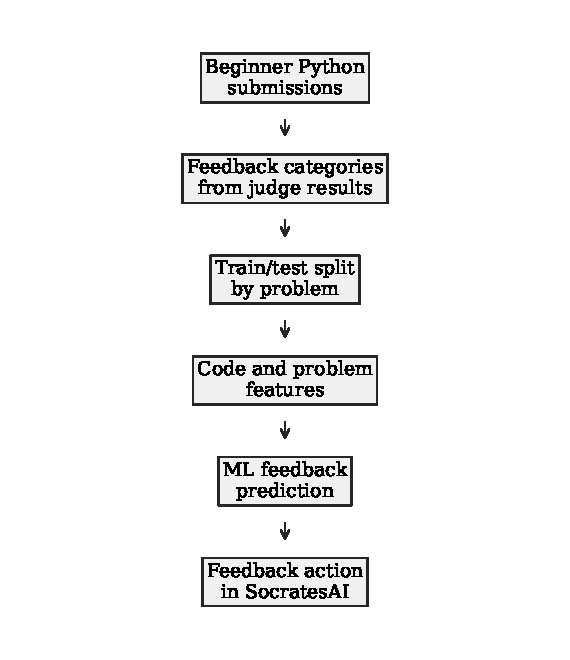
\includegraphics[width=0.58\textwidth]{figures/Figure1_ml_pipeline.pdf}
\caption{Pipeline from public programming submissions to the feedback prediction service used in SocratesAI. Test problems are kept separate from training problems to check whether the model generalizes beyond known tasks.}
\label{fig:pipeline}
\end{figure}

\begin{figure}[H]
\centering
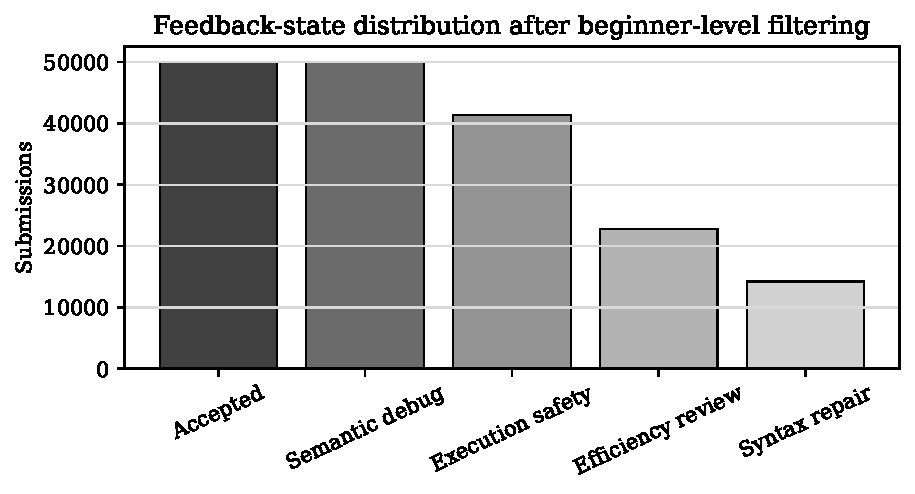
\includegraphics[width=0.74\textwidth]{figures/Figure2_state_distribution.pdf}
\caption{Distribution of feedback states after beginner-level filtering and class capping.}
\label{fig:distribution}
\end{figure}

\section{\large Results}

The model comparison is shown in Table \ref{tab:results} and Figure \ref{fig:ablation}. The majority baseline is poor under macro $F_1$ because it ignores four of the five states. Context and static metrics alone improve the score only modestly. Source code is more informative: the source-code model reaches macro $F_1=0.426$ and balanced accuracy $0.425$ on test problems that were not used during training. This result is not high enough for autonomous tutoring, but it is clearly above the majority baseline and shows that code structure contains a real feedback signal.

The strongest result is obtained when run results are added. The code-and-run model reaches macro $F_1=0.814$ and balanced accuracy $0.821$. This does not mean the mentor should simply repeat the judge result. The point is more specific: a real-time mentor that has access to test execution should use that information as a core modelling signal, not only as a final grading result.

\begin{table}[H]
\centering
\small
\caption{Model performance on the held-out problem set.}
\label{tab:results}
\begin{tabular}{|l|r|r|r|r|}
\hline
{\bf Model} & {\bf Accuracy} & {\bf Balanced acc.} & {\bf Macro $F_1$} & {\bf Weighted $F_1$} \\
\hline
Majority baseline & 0.2716 & 0.2000 & 0.0854 & 0.1161 \\
Context metrics & 0.3342 & 0.3483 & 0.3102 & 0.3040 \\
Source code & 0.4051 & 0.4248 & 0.4262 & 0.4045 \\
Source + context & 0.4039 & 0.4240 & 0.4121 & 0.3941 \\
Code + run results & 0.7808 & 0.8207 & 0.8137 & 0.7763 \\
\hline
\end{tabular}
\end{table}

\begin{figure}[H]
\centering
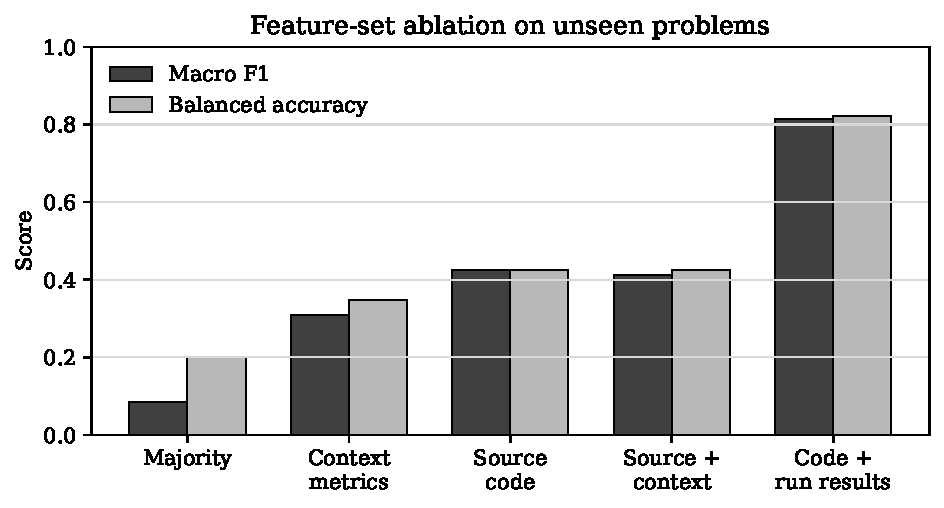
\includegraphics[width=0.78\textwidth]{figures/Figure3_feature_set_comparison.pdf}
\caption{Feature-set ablation. Source code improves over context metrics, while run results substantially improve the reliability of the decision layer.}
\label{fig:ablation}
\end{figure}

The per-class scores in Table \ref{tab:perclass} give a more useful picture than the aggregate metrics alone. The source-code model is strongest on syntax repair and efficiency review, which is reasonable because syntax fragments and code shape are visible before execution. It is weaker on accepted and semantic-debug states. This is also expected: two solutions may look structurally similar while one fails on a hidden corner case. The code-and-run model almost solves accepted, efficiency-review, and syntax-repair detection, but semantic debugging remains difficult because wrong-answer submissions and runtime-related submissions can both pass some tests and fail later.

\begin{table}[H]
\centering
\small
\caption{Per-class $F_1$ for the source-code model and the code-and-run model.}
\label{tab:perclass}
\begin{tabular}{|l|r|r|}
\hline
{\bf Feedback state} & {\bf Source code} & {\bf Code + run results} \\
\hline
Accepted & 0.3803 & 0.9157 \\
Semantic debug & 0.4116 & 0.6099 \\
Execution safety & 0.3501 & 0.6114 \\
Efficiency review & 0.4398 & 0.9712 \\
Syntax repair & 0.5490 & 0.9602 \\
\hline
\end{tabular}
\end{table}

Figure \ref{fig:confusion} gives the error classification view for the source-code model. The matrix is row-normalized, so each row shows how submissions from one true feedback state were classified. The diagonal cells are correct predictions, while the other cells show which states the model confuses. This is important for a mentor because different errors require different feedback. For example, accepted submissions are often confused with semantic debugging, and execution-safety cases are spread across accepted, semantic-debug, and efficiency-review predictions. This means that source code alone can notice useful patterns, but it cannot always separate a correct solution from a solution that fails only on hidden tests. Syntax repair and efficiency review are more separable because syntax form and repeated loop or complexity patterns are more visible in the code text.

\begin{figure}[H]
\centering
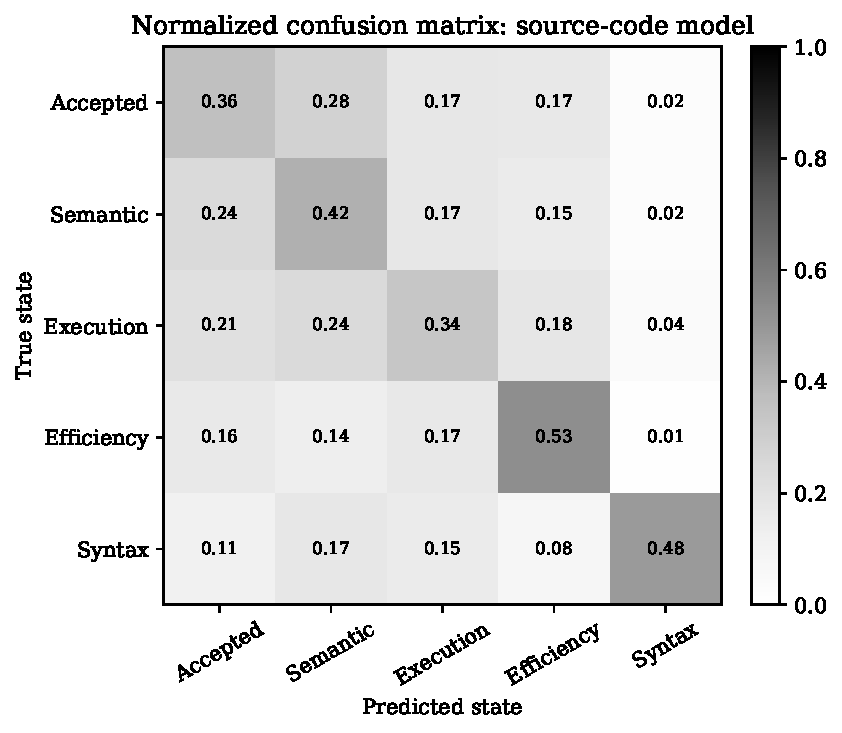
\includegraphics[width=0.69\textwidth]{figures/Figure4_confusion_matrix.pdf}
\caption{Error-classification matrix for the source-code model. Values are normalized by true feedback state; off-diagonal cells show which mentoring states are confused.}
\label{fig:confusion}
\end{figure}

\begin{figure}[H]
\centering
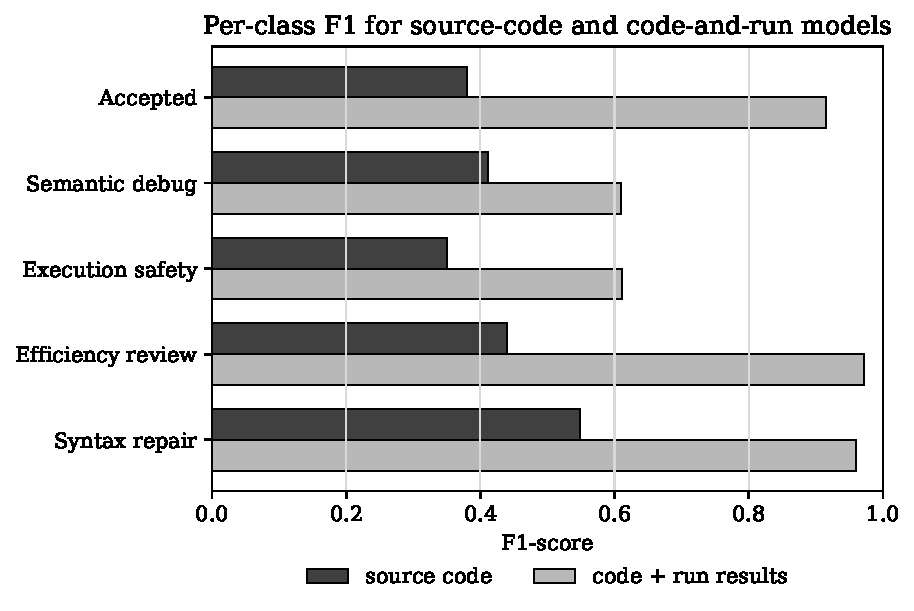
\includegraphics[width=0.78\textwidth]{figures/Figure5_per_class_f1.pdf}
\caption{Per-class $F_1$ comparison between the source-code model and the code-and-run model.}
\label{fig:perclass}
\end{figure}

The source-context result is also useful. Adding tags, rating, and static metrics did not improve macro $F_1$ over the source-code model. When test problems are kept separate from training problems, broad context does not replace source evidence; in SocratesAI it is better used to shape feedback wording or select follow-up questions.

\section{\large Integration into a virtual mentor}

In SocratesAI, the trained model is intended to sit between code analysis and feedback generation. The backend collects the submitted code, task context, and available run results. The ML service returns a feedback state and confidence scores. The feedback layer then uses that state to choose a bounded intervention style.

The integration point is deliberately small. In the implemented prototype the Python service exposes a \hbox{/predict-mentor-state} endpoint. A mentor request is represented as a JSON feature vector containing the source code, problem metadata, and optional execution measurements. The ML service returns a predicted state such as \hbox{syntax\_repair} or \hbox{efficiency\_review}, together with class scores, confidence, and the mapped feedback action. The Java backend uses the action for feedback generation and stores the predicted state and confidence in the \hbox{interaction\_logs} table. In this design the model does not need to write code for the student and does not need to expose the training dataset at runtime.

This design has two modes. In a source-only mode, the mentor can make an early estimate while the student is still editing. The results show that this mode should be treated as tentative: it can detect some syntax and structural signals, but it is not reliable enough to be the only evidence. In a code-and-run mode, the mentor uses test-run evidence and becomes much more reliable. This fits a practical workflow for first-year programming: the student writes code, runs or submits it, and receives a short intervention tied to the observed failure type.

The model does not need to produce the final hint text. Its task is to decide the pedagogical route. For example, a high-confidence efficiency-review prediction can lead to a complexity-oriented prompt; a syntax-repair prediction can lead to a localized language-form hint; a low-confidence semantic-debug prediction can trigger a cautious question asking the student to compare expected and actual output. This separation is important because it keeps the modelling problem measurable.

The final wording is produced after the feedback state is selected. In the current prototype, the feedback generation layer can use a large language model to phrase the response in natural language, but the prompt is bounded by the selected action and by safety rules: it should not provide a full solution, should not rewrite the student's program, and should keep the hint tied to the detected state. In other words, the LLM is used as a phrasing component, not as the main decision-maker. If the ML layer predicts \hbox{syntax\_repair}, the message should point to a local language-form problem; if it predicts \hbox{efficiency\_review}, the message should ask about complexity or repeated work; if confidence is low, the message should be more careful and question-based. Figure \ref{fig:interface} shows how this appears in the SocratesAI interface.

\begin{figure}[H]
\centering
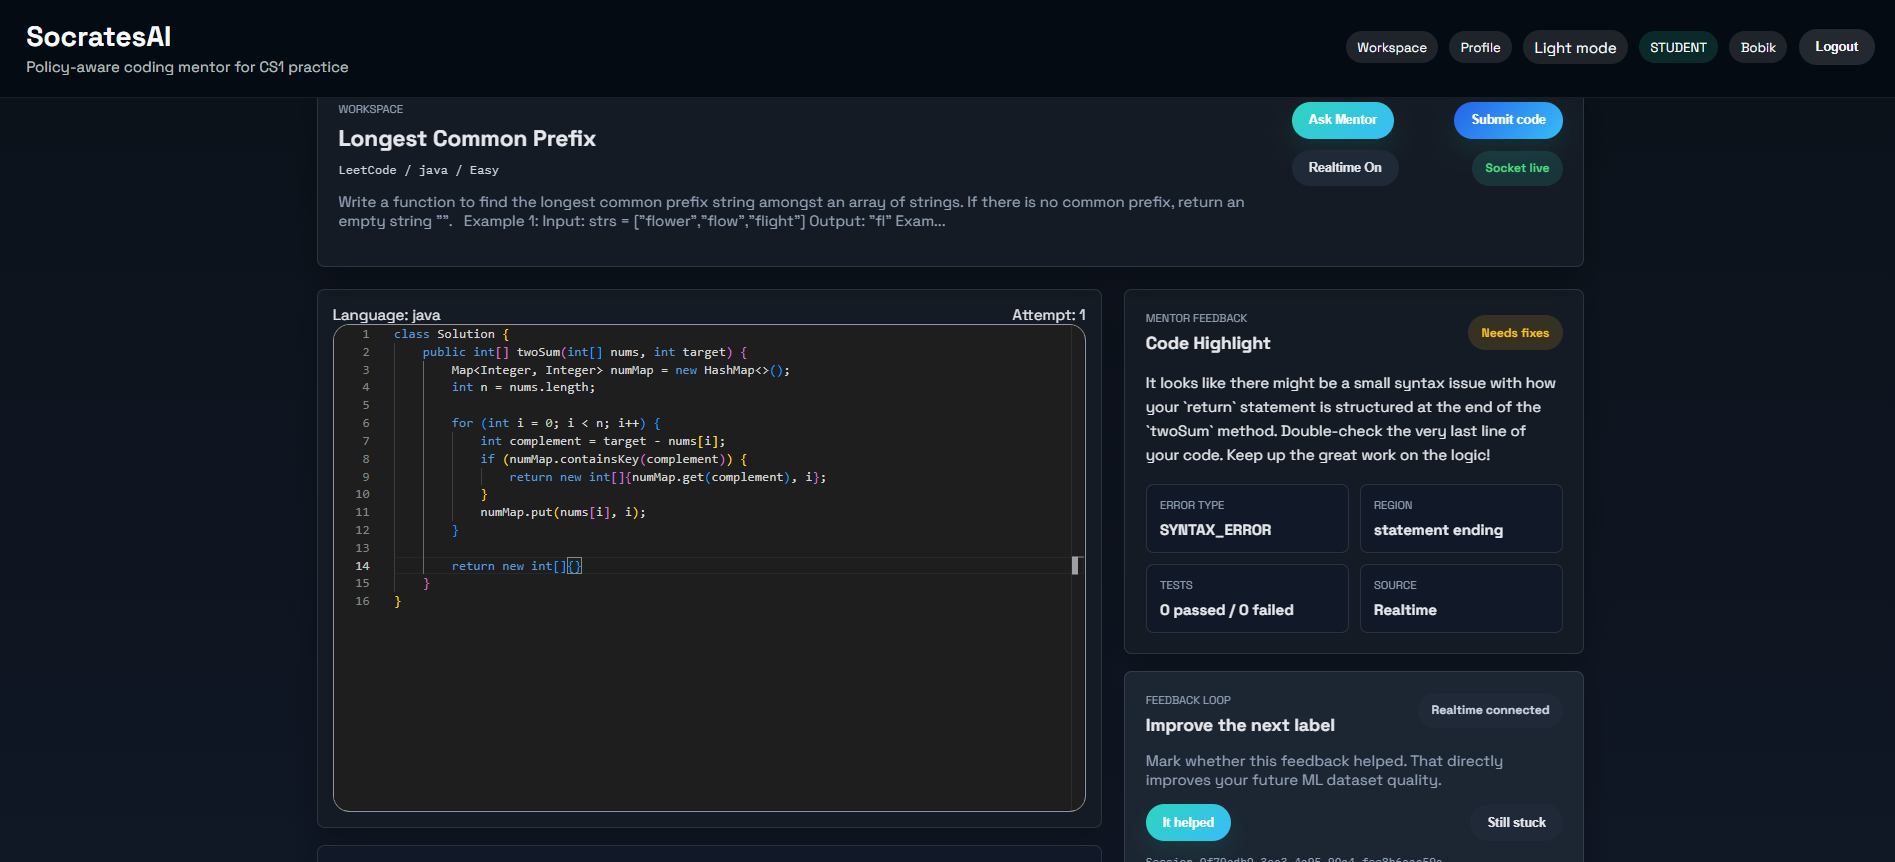
\includegraphics[width=0.86\textwidth]{figures/interface.png}
\caption{SocratesAI interface with model-guided feedback shown next to the student's code. The interface demonstrates how the predicted feedback state is turned into a short hint or question; it is not itself the evaluated ML result.}
\label{fig:interface}
\end{figure}

\section{\large Discussion and limitations}

The results support a restrained conclusion. A machine learning model can learn meaningful feedback-state signals from real programming submissions, but source code alone is not enough for reliable tutoring under unseen problems. Run results change the problem substantially. This is not a weakness of the experiment; it is a design lesson. A virtual mentor that ignores passed tests, runtime, and memory is throwing away exactly the evidence that helps separate failure modes.

There are also limitations. First, Codeforces outcomes are objective judge results, not teacher-written pedagogical labels. They define the feedback state, but they do not determine the best wording of the feedback. Second, Codeforces beginner-rated problems are only a proxy for first-year programming tasks. They are small and algorithmic, while classroom CS1 tasks may include style, decomposition, and explanation goals. Third, this paper uses Python submissions, whereas the SocratesAI prototype also targets Java practice. The model formulation is portable, but a Java-specific dataset is needed before claiming language-specific deployment quality. Fourth, the class mapping is deliberately compact. A future classroom model should distinguish finer semantic causes such as off-by-one errors, wrong invariant, input parsing mistakes, and missing edge cases.

These limitations are acceptable for the present stage because the paper is not claiming a finished educational product. It provides a stronger empirical base for the ML part of a virtual mentor and identifies where the next research step should be. The \hbox{interaction\_logs} table is therefore not replaced by the external dataset. It becomes the target-domain evaluation source: each real SocratesAI interaction can keep the model prediction, the selected action, and the student's later feedback outcome.

The most important practical implication is that a source-only mentor should be cautious. It can be useful for early warning and lightweight guidance, but the results do not justify treating it as an authoritative diagnosis. Once run results are available, the model becomes much closer to a reliable decision layer. Therefore, in a classroom system, the predicted state should be combined with confidence thresholds: high-confidence states can trigger direct bounded feedback, while low-confidence states should lead to a question or to a request for another test run.

\section{\large Conclusion}

This paper reframed virtual mentoring in introductory programming as a supervised machine learning problem over feedback states. Using 178414 real Python submissions from beginner-level Codeforces problems, the study showed that source-code features are informative but incomplete when the test problems are unseen during training. The source-code model achieved macro $F_1=0.426$, while the code-and-run model achieved macro $F_1=0.814$. The main conclusion is practical: a high-quality virtual mentor should not rely only on generated explanations or static code appearance. It should learn a feedback prediction model and use run results as a central signal for personalized intervention.

Future work will move in three directions: collecting classroom submissions from first-year students, extending the taxonomy from broad feedback states to finer debugging causes, and evaluating whether model-driven state selection improves students' ability to recover from failed attempts without receiving full solutions.

\section*{\large Acknowledgement}
The authors thank the course instructors and reviewers whose feedback helped narrow the project from a general virtual mentor prototype to a more focused machine learning study.

\begin{thebibliography}{99}
\thispagestyle{myheadings}
\vspace*{0mm} \itemsep=-2pt
\footnotesize

\bibitem{Messer2024} Messer M., Brown N.C.C., Kolling M., Shi M., {\it Automated grading and feedback tools for programming education: a systematic review}, ACM Trans. Comput. Educ., 24.1 (2024), Article 10.

\bibitem{Kumar2025} Kumar S.S., Lones M.A., Maarek M., Zantout H., {\it Navigating the landscape of automated feedback generation techniques for programming exercises}, ACM Trans. Comput. Educ., 25.4 (2025), Article 54.

\bibitem{Denny2024} Denny P., MacNeil S., Savelka J., Porter L., Luxton-Reilly A., {\it Desirable characteristics for AI teaching assistants in programming education}, Proc. ITiCSE 2024, Association for Computing Machinery, 2024, 408--414.

\bibitem{Ahamed2025} Ahmed U.Z., Sahai S., Leong B., Karkare A., {\it Feasibility study of augmenting teaching assistants with AI for CS1 programming feedback}, Proc. ACM SIGCSE TS 2025, Association for Computing Machinery, 2025, 11--17.

\bibitem{CodeAid2024} Kazemitabaar M., Ye R., Wang X., Henley A.Z., Denny P., Craig M., Grossman T., {\it CodeAid: evaluating a classroom deployment of an LLM-based programming assistant that balances student and educator needs}, Proc. CHI 2024, Association for Computing Machinery, 2024, Article 650.

\bibitem{Iris2024} Bassner P., Frankford E., Krusche S., {\it Iris: an AI-driven virtual tutor for computer science education}, Proc. ITiCSE 2024, Association for Computing Machinery, 2024, 394--400.

\bibitem{Sheese2024} Sheese B., Liffiton M., Savelka J., Denny P., {\it Patterns of student help-seeking when using a large language model-powered programming assistant}, Proc. ACE 2024, Association for Computing Machinery, 2024, 49--57.

\bibitem{Marwan2022} Marwan S., Akram B., Barnes T., Price T.W., {\it Adaptive immediate feedback for block-based programming: design and evaluation}, IEEE Trans. Learn. Technol., 15.3 (2022), 406--420.

\bibitem{Pedregosa2011} Pedregosa F. et al., {\it Scikit-learn: machine learning in Python}, J. Mach. Learn. Res., 12 (2011), 2825--2830.

\bibitem{Weinberger2009} Weinberger K., Dasgupta A., Langford J., Smola A., Attenberg J., {\it Feature hashing for large scale multitask learning}, Proc. ICML 2009, Association for Computing Machinery, 2009, 1113--1120.

\bibitem{MatrixStudio2026} MatrixStudio, {\it Codeforces-Python-Submissions}, Hugging Face dataset repository, accessed 30 May 2026. \url{https://huggingface.co/datasets/MatrixStudio/Codeforces-Python-Submissions}.

\end{thebibliography}

\footnotesize
\noindent
\parbox[t]{75mm}{
Koshikov Alimzhan,\\
School of Software Engineering,\\
Astana IT University, Astana, Kazakhstan,\\
Email: {\tt 225148@astanait.edu.kz}.}
\hfill
\parbox[t]{75mm}{
Tutkyshbayeva Shyryn,\\
School of Software Engineering,\\
Astana IT University, Astana, Kazakhstan,\\
Email: {\tt sh.tutkyshbayeva@astanait.edu.kz}.}

\vspace{3mm}
Received \_\_.\_\_.2026, $\> \> \> $ Accepted \_\_.\_\_.2026, $\> \> \> $ Available online \_\_.\_\_.2026.

\end{document}
